On s'intéresse à présent à l'objet de commande de plus haut-niveau \textit{CApprovisionnement} qui a pour rôle de commander l'approvisionnement des pièces. 

\begin{figure}
    \centering
    \ajustbox{trim={0.6\width} {0.5\height} 0 0, clip}{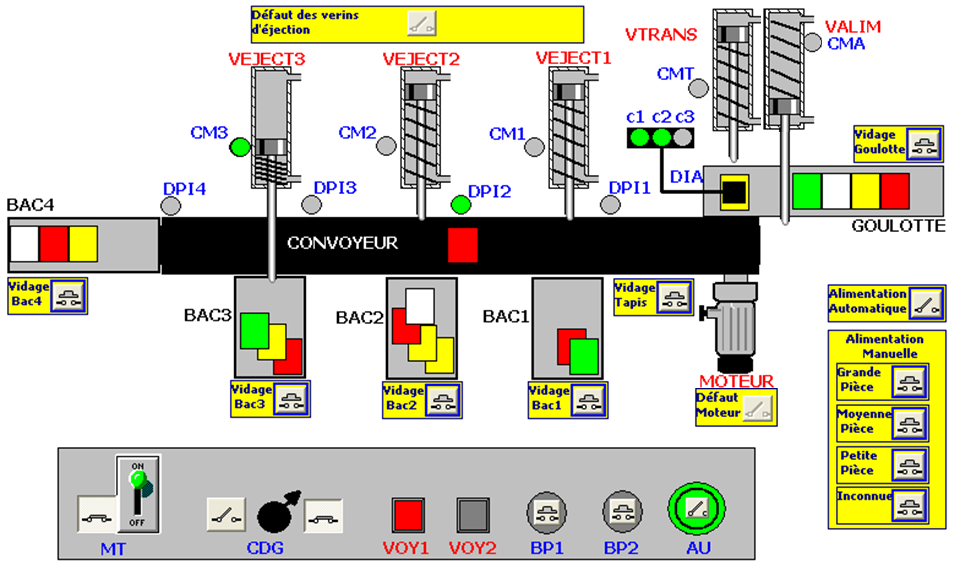
\includegraphics[width=0.8\linewidth]{tri_de_piece}}
    \caption{Système de tri de pièces}
    \label{fig:tri_de_piece}
\end{figure}

Cet objet est une agrégation de : 
\begin{itemize}
    \item Un vérin simple effet \emph{VALIM} normalement sorti, qui laisse entrer une pièce sur le poste de mesure.
    \item Un poste de mesure qui permet de mesurer la taille de la pièce.
    \item Un vérin simple effet \emph{VTRANS} normalement rentré, qui permet de transférer la pièce depuis le poste de mesure sur le convoyeur.
\end{itemize}

Les deux vérins sont commandé chacun par un objet de commande terminal \emph{oValim} et \emph{oVtrans} respectivement. Ils sont tous deux de classe \emph{CVerin} dont le type énuméré \emph{CVerinMissionIn} contient deux valeurs : \emph{RENTRER} et \emph{SORTIR}. Le type énumré \emph{CVerinEtat} contient quatre valeurs : \emph{RENTRE} , \emph{SORTI}, \emph{INTERMEDIAIRE} et \emph{DEFAUT}.

Le poste de mesure est un objet de commande de la classe \emph{CMesure}. Il s'agit d'un objet de commande extrèmement simple qui ne reçoit aucune mission mais donne sur sa propriété \emph{EtatOut} l'état de la pièce mesurée. Cette propriété est de type énuméré \emph{CMesureEtat} qui contient les valeurs : \emph{PETIT}, \emph{MOYEN}, \emph{GRAND} et \emph{DEFAUT}.

Une séquence de commande de l'approvisionnement est donnée par le diagramme d'état de la Figure \ref{fig:approvisionnement}.

\begin{figure}[h!t]
    \centering
    
    \caption{Diagramme d'état de l'approvisionnement}
    \label{fig:approvisionnement}
\end{figure}
